%Created by Fredrik Nilsson - freni169 with additions by Johan Billman - johbi142
\documentclass[12pt,a4paper]{article}
\usepackage[utf8]{inputenc}
\usepackage{alltt}
\usepackage[T1]{fontenc}
\usepackage[swedish]{babel}
\usepackage{mathtools}
\usepackage{lmodern}
\usepackage{units}
\usepackage{icomma}
\usepackage{color}
\usepackage{graphicx}
\usepackage{bbm}
\usepackage{tabularx}
\newcommand{\N}{\ensuremath{\mathbbm{N}}}
\newcommand{\Z}{\ensuremath{\mathbbm{Z}}}
\newcommand{\Q}{\ensuremath{\mathbbm{Q}}}
\newcommand{\R}{\ensuremath{\mathbbm{R}}}
\newcommand{\C}{\ensuremath{\mathbbm{C}}}
\newcommand{\rd}{\ensuremath{\mathrm{d}}}
\newcommand{\id}{\ensuremath{\,\rd}}
\usepackage{hyperref}
\usepackage[noindentafter]{titlesec}
\usepackage{color}
\usepackage{mathtools}
\usepackage{float}
\usepackage{longtable}

%Added stuff
\titleclass{\subsubsubsection}{straight}[\subsection]

\newcounter{subsubsubsection}[subsubsection]

\renewcommand\thesubsubsubsection{\thesubsubsection.\arabic{subsubsubsection}}
\renewcommand\theparagraph{\thesubsubsubsection.\arabic{paragraph}}
\renewcommand\thesubparagraph{\theparagraph.\arabic{subparagraph}}

\titleformat{\subsubsubsection}
{\normalfont\normalsize\bfseries}{\thesubsubsubsection}{1em}{}
\titlespacing*{\subsubsubsection}
{0pt}{3.25ex plus 1ex minus .2ex}{1.5ex plus .2ex}

\makeatletter
\renewcommand\paragraph{\@startsection{paragraph}{5}{\z@}%
	{3.25ex \@plus1ex \@minus.2ex}%
	{-1em}%
	{\normalfont\normalsize\bfseries}}
\renewcommand\subparagraph{\@startsection{subparagraph}{6}{\parindent}
	{3.25ex \@plus1ex \@minus .2ex}%
	{-1em}%
	{\normalfont\normalsize\bfseries}}
\def\toclevel@subsubsubsection{4}
\def\toclevel@paragraph{5}
\def\toclevel@paragraph{6}
\def\l@subsubsubsection{\@dottedtocline{4}{7em}{4em}}
\def\l@paragraph{\@dottedtocline{5}{10em}{5em}}
\def\l@subparagraph{\@dottedtocline{6}{14em}{6em}}
\makeatother

\makeatletter
\@addtoreset{subsubsubsection}{section}
\@addtoreset{subsubsubsection}{subsection}
\makeatother

\setcounter{secnumdepth}{6}
\setcounter{tocdepth}{6}
%End of new stuff


\DeclareGraphicsExtensions{.pdf,.png,.jpg}
\DeclarePairedDelimiter\abs{\lvert}{\rvert}%
\DeclarePairedDelimiter\norm{\lVert}{\rVert}%



% Swap the definition of \abs* and \norm*, so that \abs
% and \norm resizes the size of the brackets, and the 
% starred version does not.
\makeatletter
\let\oldabs\abs
\def\abs{\@ifstar{\oldabs}{\oldabs*}}
%
\let\oldnorm\norm
\def\norm{\@ifstar{\oldnorm}{\oldnorm*}}
\makeatother

\renewcommand{\abstractname}{Sammanfattning}


\setlength\parindent{0pt} %%NOINDENT



\title{TDDC74 -  Projektspecifikation}

\author{\textbf{Projektmedlemmar:}\\
Gustav Danielsson \small{gusda320@student.liu.se}\\
Marcus Dahlqvist \small{marda648@student.liu.se}\\ 
\bigskip\\ \textbf{Handledare:}\\
Jonas Wallgren {\small jonas.wallgren@liu.se}}

\date{\today}
\begin{document}
\maketitle
\newpage

\tableofcontents
\newpage

\section{Projektplanering}
Projektet går ut på att skapa ett actionspel där två till fyra spelare tävlar mot varandra. Spelet bygger på att med hjälp av tangentbordet styra varsitt flygplan på en tvådimensionell spelbana. För att vinna skall man skjuta ned motståndarnas flygplan till det att bara en spelare är kvar. Hela spelet uppdateras grafiskt i realtid.

\subsection{Kort projektbeskrivning}
Spelet bygger på ett tvådimensionellt koordinatsystem med sett från sidan. I detta plan kontrollerar två till fyra spelare varsitt flygplan, som har möjligthet att ändra sin rörelseriktning och avfyra projektiler. I spelet finns även flera utökade moment som till exempel buffar för att göra spelet intressantare(Se Användarmanual  för fullständig lista). 

\vspace{0.2cm}

Objektens rörelse beskrivs med en riktningsvektor och en hastighet, där objektet vid varje programuppdatering förflyttas i vektorsriktnig med en sträcka som beror på hastigheten.

\vspace{0.2cm}

Byggnaderna Kollisionerna bygger på att få objekten att detektera om de är nära nog ett annat objekt då de aldrig kommer dela samma flytvärde. Skulle ett objekt vara för nära aktiveras eventet för kollision som att planet störtar eller plockar upp en form av buff. \\

Alla objekt ska även vara påverkade av ett gravitationsfält som läggs över koordinatsystemet som får att alla objekt kommer att falla mot marken om denna kraft inte motverkas i form av lyftkraft i någon form. Detta leder till att om man åker rakt upp för länge kommer spelaren tappa kontrollen över flygplanet och störta för en mindre tid baserat på gravitationskraften, tills det att hastigheten har stigit igen. \\

Programmet ska kunna hantera projektiler som ska kunna skjuta ner motståndare men även andra objekt som hindrar spelarens framfart. Dessa projektiler ska inte vara påverkade av gravitation. Detta är för att underlätta siktandet men även har en projektil i ett realistiskt scenario inte är märkbart påverkad av gravitation på så korta distanser. \\

Spelet ska även innehålla olika former av bonusar som kan plockas upp. Detta ger allt från en fartökning till nytt vapen eller liknande. Dessa ska kunna påverka planets beteende och dess rörelse i koordinatsystemet.  Även ska objekt kallat entities, som kan komma i form av till exempel fåglar eller luftballonger, kunna bli nedskjutna som kommer innehålla bonusar eller bara behöver bli förstörda så att man inte kolliderar med dem. 
Planet i sig ska kunna flyga i 16 olika riktningar för att ge en mjukare svängning samt ge fler riktningar att skjuta i så att spelaren har mer möjligheter att skjuta ner motståndaren. Vi svängning ska planet följa riktningen men även vridas runt x axeln för att ge en visuellt mer realistisk bild av att plant svänger. \\

Slutligen ska spelets inställningar kunna påverkas via en huvudmeny. Inställningarna består av val av spelbana, flygplan, antal poäng till vinst mm. Samt så ska spelet kunna pausas när en knapp trycks ned, och en pausmeny öppnas. Från denna meny ska man kunna återgå till spelet, avsluta pågående omgång eller avsluta programmet helt. \\


\subsection{Utvecklingsmetodik}
Vi strävar efter att genomföra det huvudsakliga arbetet i skolan på de erhållna tiderna. Vid behov försöker vi främst utnyttja lediga tider under arbetsveckan med vid behov även göra eget arbete hemma. Då båda medlemmarna har tillgång till laptop kan arbetet ske på valfri plats. Utöver det så ses vi dagligen samt har god kontakt vilket gör att kommunikation mellan medlemmarna kan ske utan stora förhinder. \\

Koden kommer att versionshanteras med tjänsten gitlab som kommer att underlätta konflikter med koden samt så erbjuder gitlab möjligheten att gå tillbaka till äldre versioner av koden vid olösliga problem.

\subsection{Grov tidplan}
I början kommer vi huvudsakligen att arbeta tillsammans för att få en bra struktur och en gemensam grundidé att arbeta utifrån. Vi strävar att få det gemensamma arbetet över så fort som möjligt då det är effektivare att arbeta individuellt. Sen utifrån grunden kan vi börja jobba mer individuellt på kommandon och olika grafiska delar som planens utseende till menyer eller finjustera fysikmotorn. Vi kommer dock ses regelbundet för att få en bättre bild av vad den andra personen gjort. På grund av att vi ses dagligen blir det även lätt att diskutera eventuella konflikter som uppstår vid individuellt arbete. \\

Vi kommer behöva bekanta oss med att arbeta med rackets inbyggda grafikpaket för att skapa menyer och spelet i sig. Samt så behöver vi lära oss att arbeta med realtidsuppdateringar och inte skapa ett spel som upplevs allt för ryckigt i manövreringen. \\

Till halvtidsmötet ska fysikmotorn och rörelsen i koordinatsystemet vara klart så spelet är fungerande fast utan grafik. Efter mötet kommer vi fokusera på att implementera grafiken och sedan relevanta funktioner när spelet har en grafik, såsom menyer, att kunna påverka vinstkriterier och avsluta spelet från en pausmeny.

\subsection{Betygsambitioner}
Då båda är intresserade av att göra ett så bra och givande projekt som möjligt siktar vi på att nå betyg 5. Vi båda arbetade på samma ingenjörsprojekt som byggde på att skriva ett reglertekniskt program och vi vill förbättra våra förmågor i utvecklandet av program ur ett projektperspektiv. 

\section{Användarmanual}\label{Användarmanual}
Programmet är sparat som Dogfight.exe och startas genom att köra filen. Vid start öppnas en startmeny som berättar grunderna till spelet för spelarna. \\

\begin{figure}[H]
	\caption{Spelets startmeny}
	\centering
	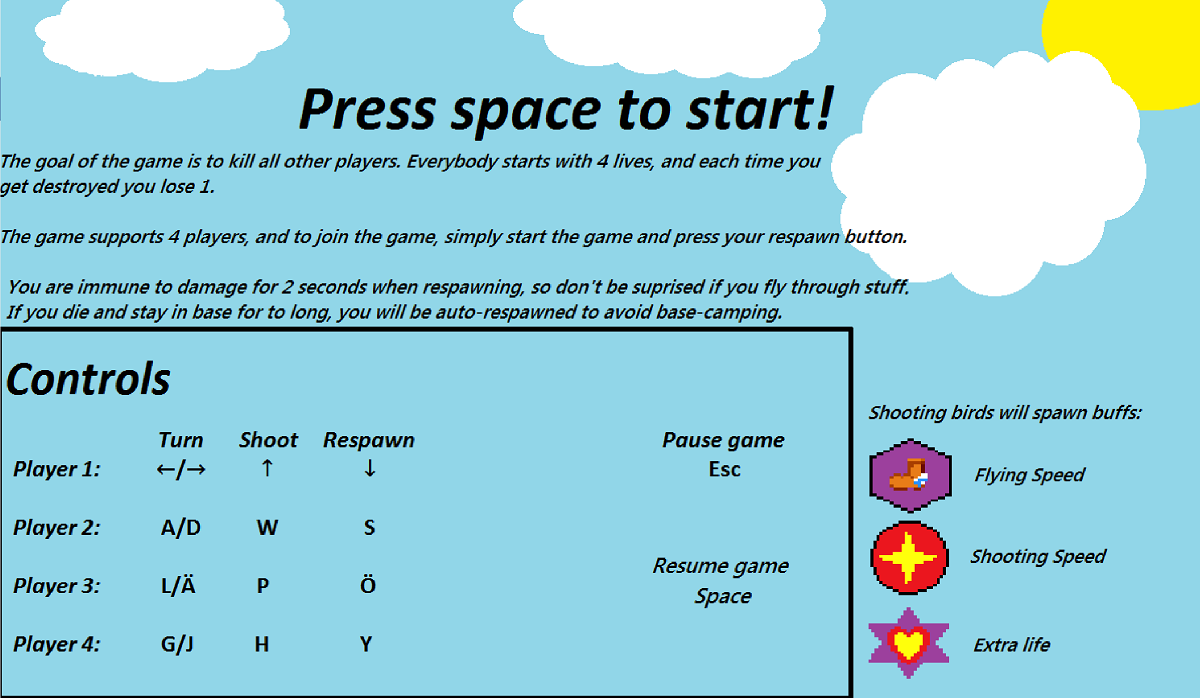
\includegraphics[width=\linewidth]{Dogfight_Menu_Example.png}
\end{figure}

Från Figur 1 kan all information som krävs för att kunna spela spelet erhållas. Alla spelarnas kontroller finns beskrivna i controls-rutan samt till höger om den en kort förklaring om hur de olika buffarna ser ut. Dessa erhålls som texten säger genom att skjuta ner fåglar. Reglerna för antal liv samt viktiga regler om hur respawning funkar erhålls ur texten över controls-rutan. Vid tryck på blanksteg genereras världen och spelarna kan då börja tävla mot varandra. \\

\begin{figure}[H]
	\caption{Hur en spelomgång kan se ut}
	\centering
	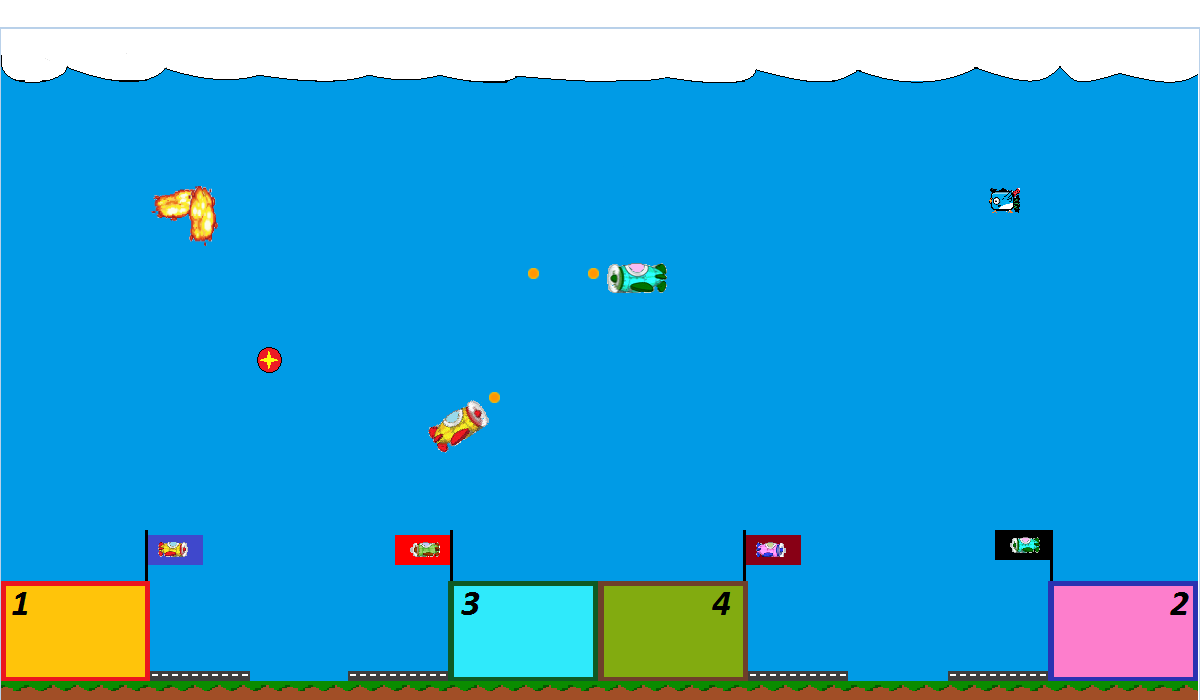
\includegraphics[width=\linewidth]{Dogfight_Run_Example.png}
\end{figure}

Under en spelomgång kommer varje spelare som nämnts tidigare tilldelas 4 liv, dock kan fler erhållas genom att skjuta ned fåglar. Fåglar kommer att genereras slumpmässigt vid spelplanens kanter och flyga tills de träffas av en projektil eller krockar i en vägg. Spelare kan flyga in i kortsidan av spelplanen och komma tillbaka på andra sidan. Detta gäller dock ej för projektiler eller fåglar, som istället försvinner från spelet. Vid kollision kommer spelare att förlora ett liv samt så kommer spelarens flagghöjd att sänkas för att representera antalet kvarstående liv. Alla spelare kommer att kunna, förutsatt att de har liv kvar, kunna återuppstå vid hangaren med deras nummer på. \\


Funktionen finns även att om en spelare väntar för länge utan att återuppstå så tvingas de återuppstå för att förhindra att någon spelare gömmer sig i hangaren.\\

Inga poäng erhålls för att skjuta ned någon utan det är en fråga om att inte krocka eller bli nedskjuten för att vinna. När alla andra spelare har slut på liv vinner den sist levande spelaren. Vid det eventuella fallet att de sista spelarna dör samtidigt räknas spelet som oavgjort.

\begin{figure}[H]
	\caption{Exempel på vinstskärm}
	\label{Win}
	\centering
	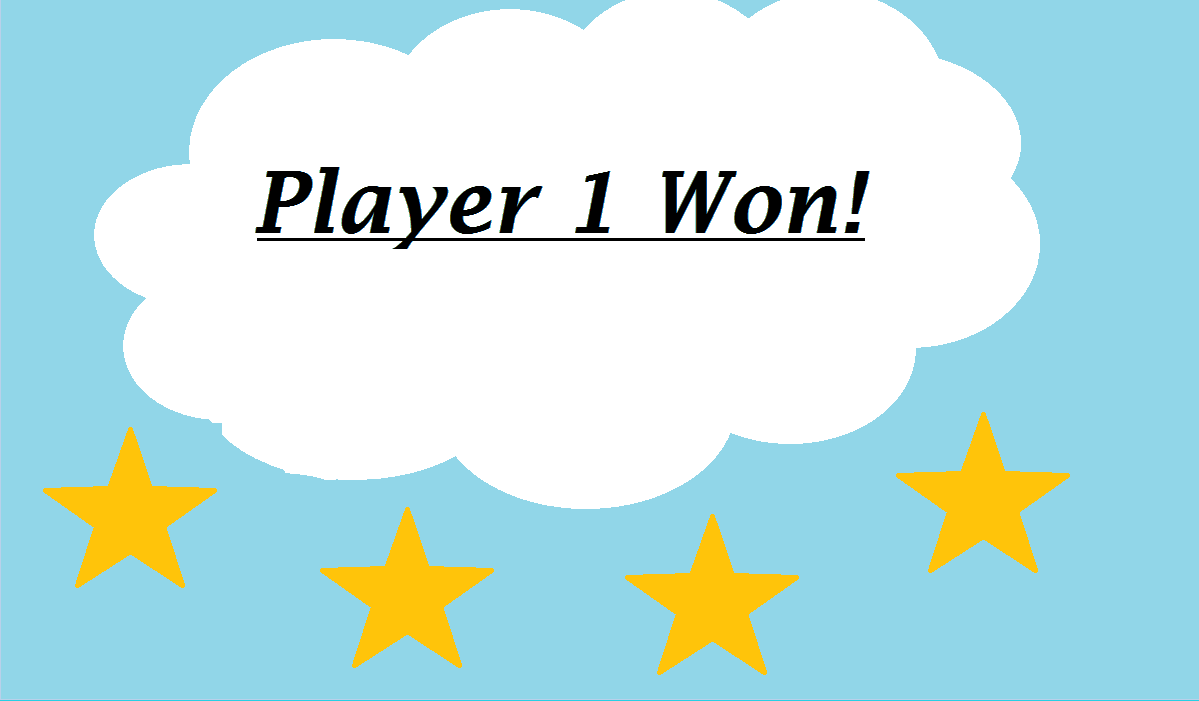
\includegraphics[width=\linewidth]{Win_Example.png}
\end{figure}

När någon spelare har vunnit kommer man till en skärm som klargör vinnaren(se figur 3), eller oavgjort om så är fallet, och för att spela en gång till behöver programmet startas om igen. Viktigt att notera är att det krävs två spelare för att ha en vinnare samt att det enda man behöver göra för att delta är att trycka på sin tangent för återuppståndelse. Detta kan göras hela tiden tills en vinnare har valts. Spelet är därför rekomenderat att spelas med minst två spelare för att få någon form av tävling, men det blir roligare med fler spelare då det blir mer hinder samt mer utmaning.

\section{Kravlista}
Här specificeras kraven för projektet. De lägre kravprioriteringarna 4-5 är inte nödvändiga, om implementeras snarare efter tillgänglig tid efter 1-3 är färdiga. 
\begin{longtable}{ | p{3.5cm} | c | c | p{3.5cm} | }
	\hline
	Krav & Prioritet & Kategori & Kommentar  \\ 
	\hline
	Världen ska byggas på ett tvådimensionellt koordinatsystem & 1 & Fysikmotor & \\
	\hline
	Det skall finnas objekt som kan ändra sin position i koordinatsystemet & 1 & Fysikmotor & \\
	\hline
	Positioner skall kunna uppdateras i realtid & 1 & Fysikmotor & \\
	\hline
	Objekt skall kunna förflyttas rakt i flera olika riktningar (16+) & 1 & Fysikmotor & Antal riktningar beror på vad som ger bäst spelupplevelse \\
	\hline	
	Objekt skall kunna ha olika storlek & 1 & Fysikmotor & \\ 
	\hline
	Objekt skall kunna kollidera med varandra & 1 & Fysikmotor & Exempelvis aktivering av en buff eller krascha mot marken \\ \hline
	
	Hastigheten för objekt skall vara varierbar & 2 & Fysikmotor & \\ 
	\hline
	Ett objekt som kolliderar med vänster/högerkant skall kunna komma fram på motsatt sida & 3 & Fysikmotor & \\ \hline
	Enkel gravitiation skall kunna simuleras & 3 & Fysikmotor & Kommer ungefär fungera så att objekt som rör sig uppåt kommer att få en lägre hastighet än de som rör sig nedåt. Kommer ej vara en konstant acceleration nedåt.\\ \hline
	Spelet skall kunna simulera vind  & 5 & Fysikmotor & \\ \hline
	Det skall vara möjligt att välja olika världar med annorlunda fysik & 5 & Fysikmotor & T.ex. välja att spela på månen med lägre gravitation eller liknande\\ \hline
	Det skall finnas spelarobjekt som kan styras av spelaren & 2 & Spelelement & \\ \hline
	Det skall  finnas en möjlighet för två spelare & 2 & Spelelement & \\ \hline
	Det skall finnas icke-spelarobjekt som spelaren kan interagera med & 2 & Spelelement & \\ \hline
	Det skall finnas ett markplan längst ned i världen & 2 & Spelelement & Vissa element kommer att elimineras vid kollision med marken\\ \hline
	Det skall finnas en himmel som gör att spelaren faller & 2 & Spelelement & Fungerar som ett tak fär spelplanen\\ \hline
	Spelaren skall kunna avfyra projektil-objekt  & 2 & Spelelement & Fungerar som vapen och kommer bland annat att kunna förstöra motspelare\\ \hline
	Det ska  finnas objekt som spelaren kan kollidera med som gör att spelaren kraschar & 2 & Spelelement & \\ \hline
	Det skall finnas ett vinst/förlustkriterie & 2 & Spelelement & I sin grund att skjuta ned motspelaren\\ \hline
	Vid för låg hastighet riktad uppåt skall spelarobjektet kunna förlora kontrollen & 2 & Spelelement & Planet faller rakt ned utan kontroll till en viss hastighet uppnås, varvid spelaren kan börja styra igen\\ \hline
	Om två spelare kolliderar med varandra skall båda krascha & 3 & Spelelement & \\ \hline
	Det skall finnas en plats där spelaren kan återuppstå & 3 & Spelelement & Kommer att vara i form av en landningsbana vid marken\\ \hline
	Vinst- och förlustfunktionen ska utökas så att varje spelare har flera liv & 3 & Spelelement & \\ \hline
	Spelaren skall vara immun mot skada en kort tid efter återuppståndelse & 3 & Spelelement & För att undvika att motspelaren missbrukar den överlägsna positionen\\ \hline
	Spelaren skall ha tillgång till en aktiverbar hastighetsboost & 3 & Spelelement & Kommer att ha en tidsbegränsad aktiveringsfrekvens, som eventuellt kan förändras av bonusar\\ \hline
	Det skall finnas bonusar som spelaren kan aktivera & 3 & Spelelement & Kommer att göra saker som att öka maxhastighet, skjuthastighet m.m.\\ \hline
	Vid krasch ska spelaren störta mot marken, fortfarande med kollision & 4 & Spelelement & Det vill säga att andra objekt fortfarande kan kollidera med den till den når marken\\ \hline
	Det skall finnas stöd för upp till 4 spelare & 4 & Spelelement & \\ \hline
	Det skall vara möjligt att välja olika vinstkriterier & 5 & Spelelement & Detta skulle kunna vara: Tidsbegränsningar, fler liv, lagspel för 4 spelare.\\ \hline
	Man skall kunna starta spelet med 1 kommando & 1 & Användargränssnitt & Kommandot skall öppna en startmeny\\ \hline
	Det skall finnas en startmeny & 2 & Användargränssnitt & Skall innehålla instruktioner, start av spel och senare möjlighet att justera spelinställningar\\ \hline
	Det skall finnas en undermeny för instruktioner & 2 & Användargränssnitt & Här visas kontroller, vilka buffs som finns, och hur spelet går till\\ \hline
	Det skall finnas en knapp som startar huvudspelet i menyn & 2 & Användargränssnitt & \\ \hline
	Det skall finnas en knapp som avslutar spelet i huvudmenyn & 2 & Användargränssnitt & \\ \hline
	Huvudspelet skall kunna styras endast med ett tangentbord & 2 & Användargränssnitt & Kontrollerna som finns kommer att vara: Ändring av färdelseriktning medsols och motsols, avfyrning av vapen och aktivering av hastighetsboost\\ \hline
	Det skall finnas en knapp som avslutar spelet i huvudspelet & 2 & Användargränssnitt & \\ \hline
	Det skall finnas en knapp som pausar spelet & 3 & Användargränssnitt & i denna meny skall man kunna avsluta spelet eller återvända till huvudmenyn\\ \hline
	Menyn skall kunna navigeras endast med mus & 3 & Användargränssnitt & \\ \hline
	Det ska vara möjligt att själv ändra kontrollbindningarna i menyn & 5 & Användargränssnitt & \\ \hline
	Huvudspelet skall vara grafiskt implementerat & 2 & Grafik & \\ \hline
	Alla menyer skall vara grafiskt implemenerade & 3 & Grafik & \\ \hline
	Det skall finnas en indikator för antalet kvarstående liv & 3 & Grafik & \\ \hline
	Det skall finnas en indikator för hastighet & 4 & Grafik & \\ \hline
	Det skall finnas en indikator för kvarvarande tid till hastighetsbonus & 4 & Grafik & \\ \hline
	Det skall finnas en indikator för aktiverade bonusar & 5 & Grafik & \\ \hline
	Det skall finnas stöd för ljud i spelet & 4 & Övrigt & \\ \hline
	Ljud skall implementeras i huvudspelet & 4 & Övrigt & \\ \hline
	Det skall finnas musik i menyerna & 5 & Övrigt & \\ \hline
	Vid spelets slut skall statistik för matchen visas & 5 & Övrigt & Antal avfyrade skott, antal liv vid spelets slut, tidsåtgång, aktiverade bonusar, m.m.\\ \hline
\end{longtable}

\section{Implementation}
Här beskrivs processen under ett programvarv, de datatyper som används av programmet, samt hur alla objekt i världen är behandlade och representerade.

\subsection{Processbeskrivning}
Spelet uppdateras i realtid med uppdateringsfrekvensen 16ms. När spelet startas från början kommer spelaren till huvudmenyn, och det enda kommando som finns tillgängligt här är att trycka på blanksteg, vilket för spelaren till själva spelet och huvudproceduren startar. Huvudproceduren utför ett antal kommandon stegvis för att sedan börja om igen, förutsatt att ingen har vunnit eller pausat spelet. En uppdateringssekvens ser ut som följande:

\begin{description}
	\item [  I. Indata] Det första som händer i huvudloopen är att indata kontrolleras, vilken kommer i form av tangenttryck från spelarna. Om pausknappen då är intryckt, så fryses uppdateringsloopen och programmet väntar på att startknappen ska tryckas ned. Om detta inte är fallet så sätts variabler för alla nedtryckta knappar att spelaren försöker utföra ett kommando. Om en knapp har blivit släppt sedan senaste uppdateringen, så sätts istället denna variabel till falsk.
	
	\item [  II. Rörelser] När all indata blivit hämtad, hanteras rörelser. Först kollas om spelarna har försökt svänga, och om de har det kollas sedan om de är tillåtna att göra detta. Efter detta så roteras alla spelare om de var tillåtna. Efter detta förflyttas alla flygande objekt framåt längs deras riktningsvektor med avståndet som beror på deras hastighet.
	
	\item [  III. Kollisioner] Efter detta testas alla flygande objekt om de kolliderar med något annat objekt eller världen. Om så är fallet så utförs då rätt åtgärd för kollisionen.


	\item [  IV. Skapandet av projektiler] Nästa steg är att testa om vilka spelare som försöker skjuta, och om de är tillåtna skapa en projektil framför nosen på spelaren.
	
	\item [  V. Skapandet av spelare] Här kollas om en spelare försöker återuppstå, och skapar dem förutsatt att de är tillåtna. Här kollas även om spelaren varit död för lång tid, och om så är fallet tvingas spelaren återuppstå oavsett.
	
	\item [  VI. Skapandet av fåglar] Här kollas först om en fågel bör skapas vid sidan av skärmen, och om så är fallet skapas den på en slumpmässigt framtagen position.
	
	\item [  VII. Grafik] Nu har hela världen uppdaterats, och då ritas grafiken ut för spelaren att se.
	
	\item [  VIII. Vinst] Sista steget är att kolla om en vinst har inträffat. Om så är fallet går spelet ut ur loopen, och annars så börjar programmet om igen på steg I.
		
\end{description}

\subsection{Abstrakta datatyper}
 OBS!: allt under VÄRLDEN är gammalt och ska göras om.

\subsubsection{Vektorer}

Lorem ipsum

\subsubsection{Cirklar}

Lorem ipsum

\subsubsection{Rektanglar}

Lorem ipsum

\subsubsection{Världen}

Här beskrivs hur världen och dess objekt är definierade och behandlade.

\subsubsubsection{Geometri}
Världen är representerad som ett tvådimensionellt koordinatsystem med origo i nedre vänstra hörnet på skärmen, och har positiv x-led åt höger, samt positiv y-led uppåt. Världen begränsas uppåt, nedåt och åt sidorna av linjer, som fungerar som gränser för att objekt inte ska färdas utanför skärmen. Om någon av dessa linjer korsas av ett objekt försvinner objektet, förutom fallet då en spelare passerar sidolinjen, då spelaren istället förflyttas till motsatt sida. I världen finns även 4 byggnader i form av hangarer, vilka är representerade som stationära rektanglar.

\subsubsubsection{Objekthantering}

Världen håller även koll på objekten som befinner sig i världen. Objekten är sparade i fyra olika listor, som alla behandlas på olika sätt:

\begin{description}
	\item [  I. Byggnader] Här sparas de fyra hangarerna, och denna används för att testa om något av de flygande objekten har kolliderat med någon av byggnaderna.
	
	\item [  II. Flygande enheter] Här sparas alla flygande objekt, det vill säga spelare, fåglar, buffar och projektiler. Objekten i denna lista är de enda objekt som kan förflytta sig, och därför även de som aktivt kan kollidera med andra objekt. Därför används denna lista för rörelser, kollisioner samt utritning av dessa objekt.
	
	\item [  III. Kroppar] Denna lista innehåller alla objekt som nyligen dött, och syftet med listan är att spara alla dessa objekts position så att deras kropp kan ritas ut.
	
	
	\item [  IV. Aktiva spelare] Denna lista spar alla spelare som aktivt har anslutit sig till spelet, det vill säga upstått första gången. Denna används för att hantera vinst och utritning av flaggor.
\end{description}

\subsubsubsection{Variabelhantering}

Världen håller även reda på några variabler som beskriver spelets nuvarande status. De variabler som finns håller koll på om spelet har startat, om spelet är över, om spelet är pausat, om en fågel bör skapas, samt om någon precis dött. Att en fågel ska skapas är begränsad av en slumpmässig tid från att den förra fågeln skapades, och om den ska skapas så görs detta på en slumpmässigt framtagen position vid spelplanens kant. Variabeln för att någon precis dött används för att se om detta resulterade i att någon vann spelet.

\subsubsection{Flying-unit}
Datatypen \textbf{flying-unit} kommer att vara en överklass till alla flygande objekt, det vill säga spelare, hinder(exempelvis fåglar) och bonusar. Denna datatyp kommer även att representera projektiler som spelaren avfyrar, men då dessa projektiler inte har några extra egenskaper utöver de som beskrivs av \textbf{flying-unit}, så kommer denna klass att användas för att beskriva dem direkt.
\vspace{0.2cm}

\begin{tabular}{| c | c | p{8.3cm} |}
	\hline
	\textbf{Metod} & \textbf{Variabel} & \textbf{Beskrivning} \\
	\hline
	 
	 get-size & - & Returnerar bonusens storlek. \\
	 \hline
	 get-coordinates & - & Returnerar var spelaren befinner sig just nu. \\
	 \hline
	 get-direction & - & Returnerar åt vilken riktning spelaren är riktad åt i radianer.\\
	 \hline
	 get-speed & - & Returnerar vilken hastighet spelaren rör sig i.\\
	 \hline
	 set-coordinates! & \small\textbf{X Y} & Ändrar spelarens koordinater. \\
	 \hline
	 set-direction! & \small\textbf{angle} & Ändrar spelarens riktning. \\
	 \hline
	 set-speed! & \small\textbf{speed} & Ändrar spelarens hastighet. \\
	 \hline
\end{tabular}


\subsubsubsection{Player}
Datatypen \textbf{player} kommer att vara en klass som beskriver spelarobjekt, och kommer utöver de allmänna variablerna hos flygande objekt även att innehålla spelarobjektets unika egenskaper.

\vspace{0.2cm}

\begin{tabular}{| c | c | p{7.8cm} |}
	\hline
	\textbf{Metod} & \textbf{Variabel} & \textbf{Beskrivning} \\
	\hline
	
	get-size & - & Returnerar spelarens storlek \\
	\hline	
	get-max-speed & - & Returnerar spelarens tillåtna maxhastighet. \\
	\hline
	get-lives & - & Returnerar spelarens antal kvarstående liv \\
	\hline
	is-defeated? & - & Returnerar \#t om spelaren blivit besegrad, det vill säga inga liv kvar, och annars \#f. \\
	\hline
	can-fire? & - & Returnerar \#t om spelaren är tillåten att skjuta, annars \#f.\\
	\hline
	can-speedboost? & - & Returnerar \#t om spelaren är tillåten att använda speedboost, annars \#f. \\
	\hline
	is-plunging? & - & Returnerar \#t om spelaren har förlorat kontrollen på grund av för låg fart, eller kolliderat med toppen av spelplanen, annars \#f. \\
	\hline
	is-dead? & - & Returnerar \#t om spelaren är ur spel på grund av krasch, annars \#f. \\
	\hline
	set-max-speed! & \small\textbf{speed} & Ändras spelarens tillåtna maxhastighet. \\
	\hline
	set-lives! & \small\textbf{lives} & Sätter spelarens antal liv. \\
	\hline
	toggle-defeated! & - & Växlar om spelaren har blivit besegrad. \\
	\hline
	toggle-fire! & - & Växlar om planet är tillåtet att skjuta.\\
	\hline
	toggle-speedboost! & - & Växlar om planet är tillåtet att använda speedboost. \\
	\hline
	toggle-plunging! & - & Växlar om planet har förlorat kontrollen. \\
	\hline
	toggle-dead! & - & Växlar om spelaren är ur spel. \\
	\hline
	
\end{tabular}

\subsubsubsection{Buff}
Datatypen \textbf{buff} kommer att vara en klass som beskriver bonusobjekt, och kommer utöver de allmänna variablerna för flygande objekt även beskriva vilken typ av bonus det är. \\

\begin{tabular}{| c | c | p{8.2cm} |}
	\hline
	\textbf{Metod} & \textbf{Variabel} & \textbf{Beskrivning} \\
	\hline

	get-bonus-type & - & Returnerar vilken typ av bonus objektet är. \\
	\hline
	
\end{tabular}

\subsubsubsection{Entities}
datatypen \textbf{entities} kommer att vara en klass som beskriver flygande objekt som inte styrs av spelaren(exempelvis fåglar), och kommer förutom de allmäna egenskaperna för flygande objekt att beskriva de unika egenskaperna för dessa objekt. \\

\begin{tabular}{| c | c | p{9.5cm} |}
	\hline
	\textbf{Metod} & \textbf{Variabel} & \textbf{Beskrivning} \\
	\hline
	
	get-buff & - & Returnerar vilken typ av bonusobjekt som detta objekt lämnar efter sig vid kollision med en projektil, eller \#f om ingen lämnas.\\
	\hline
	
\end{tabular}

\subsubsection{World}
Datatypen \textbf{world} kommer att vara en klass som beskriver alla icke-rörliga kollisionsobjekt på spelplanen, det vill säga marken, himlen och landningsbanorna. \\

\begin{tabular}{| c | c | p{8cm} |}
	\hline
	\textbf{Metod} & \textbf{Variabel} & \textbf{Beskrivning} \\
	\hline
	
	get-coordinates & - & Returnerar vilka koordinater objektet har. \\
	\hline
	get-size & - & Returnerar objektets storlek. \\
	\hline
	get-type & - & Returnerar typen av kollisionsobjekt. Detta för att avgöra vilken åtgärd som ska utföras vid kollison, det vill säga förlust av kontroll för himmlen och krasch för mark och landningsbana. \\
	\hline
\end{tabular}

\subsubsection{Background}
Datatypen \textbf{background} kommer att beskriva den bakgrund vilket spelet spelas över, och även bakgrunden i menyerna. Denna kommer att vara statisk under spelets gång, och kommer därför bara att behöva uppdateras vid uppstart och när man går till menyn.

\vspace{0.2cm}

\begin{tabular}{| c | c | p{7cm} |}
	\hline
	\textbf{Metod} & \textbf{Variabel} & \textbf{Beskrivning} \\
	\hline
	
	choose-background & background & Ändrar vilken bakgrund som visas, exempelvis meny- eller huvudspelsbakgrund.\\
	\hline
	render & - & Börjar visa bakgrunden på skärmen. \\
	\hline
	hide & - & Slutar visa bakgrunden på skärmen. \\
	\hline
\end{tabular}

\subsubsection{Vector}
Datatypen \textbf{vector} kommer att beskriva vektorer och punkter i koordinatsystemet, om kommer bestå av ett par där car-delen är x-värdet och cdr-delen y-värdet.

\subsubsection{Matrix}
Datatypen \textbf{matrix} kommer att beskriva matriser som används för beräkningar, och kommer att bestå av en lista, där första elementet är en lista av första raden i matrisen, andra elementet är en lista av andra raden, etcetera.


\subsection{Testning}
När det gäller tester så är det främst viktigt att rörelserna i koordinatsystemet och kollisiondetekteringen fungerar på rätt sätt. Vi kommer därför att behöva testfunktioner som avläser och skriver ut de variabler som framkommer vid ett programvarv, för att se att saker får rätt position, att kollision detekteras korrekt samt att händelser kontrolleras och utförs korrekt. Lämpligt här är att skapa en testfunktion där programmet kan uppdateras med hjälp av ett knapptryck eller kommando istället för en klocka, för att på så sätt kunna analysera varje uppdatering på detaljnivå. Man bör även i kunna sätta alla variabler manuellt i testfunktionen, för att kunna testa specifika fall enklare. \\

Tidigt i implementeringen kommer vi främst att testa så att rörelser fungerar korrekt, så att föremål får rätt position i koordinatsystemet givet en riktning och en hastighet. När detta fungerar är huvudfokus att testa kollision av objekt och i sin tur att storlekar av objekt fungerar på rätt sätt. Här finns det även viktiga speciallfall att testa, till exempel om 3 objekt kolliderar med varandra under samma programvarv, då måste någon form av händelseprioritering göras. \\

Senare i projektet kommer även grafiken att behöva testas, men då fysikmotorn då redan ska vara implementerad handlar detta främst om att se så att kollisioner och liknande inträffar synkroniserat med att de grafiska objekten kolliderar. \\

\subsection{Beskrivning av implementation}


\subsubsection{Rörelser}
I spelet har alla objekt representerats som fyrkanter eller cirklar. Detta för att deras rörelse kan uttryckas men linjär algebra. Rörelserna i koordinatsystemet är antingen förflyttning längs en vektor eller en rotation om objektet är en rektangel. \\

\subsubsubsection{Förflyttning längs vektorer}
Alla objekt som rör dig är definierade utifrån sin mittpunkt och om det är en rektangel utifrån dess hörn med. Dessa punkter är sparade i kordinatpar med x och y värden. Objekten ges även en riktning de färdas i samt en hastighet. Dessa kan liknas med den algebrans vektorbeskrivning
\begin{math}
$$\lambda$$
	\begin{pmatrix}
		x \\
		y
	\end{pmatrix}
\end{math}
där x och y är rörelsen i respektive led och $\lambda$ är vektorns längd. Vid förflyttning utnyttjas punktens x och y värde samt längden av vektorn för att sedan med enkel addition avgöra dess nya koordinater vid förflyttning. Hastigheten kan manipuleras av buffar som plockas upp och riktningen av spelarens knapptryck. \\

\subsubsubsection{Rotationer}
Rotationer rör endast rektanglarna och är en procedur som sker efter förflyttningen av objektet. Alla rektanglar är definierade utifrån en mitt punkt samt dess hörn. För att lättare kunna räkna på rotation har även alla hörn sitt korresponderande projekterat hörn. Detta är hörnen som rektangeln har efter rotation och är de hörn som kollisionshanteringen använder. Grundhörnen är inte påverkade då alla rotationer utgår från dessa hörn och roteringen sker baserat på dess hörns position. Grundhörnen är baserade på en noll radianers vinkel och är även de hörn som förflyttas längs vektorer. De projicerade hörnen bestäms efter att föremålet förflyttats. \\

All rotation utgår från en rotationsmatris 
\begin{math}
	\begin{pmatrix}
	\cos (\theta) & -\sin (\theta) \\
	\sin (\theta) & \cos (\theta)  
	\end{pmatrix}
\end{math}
där rotationen sker längs en tredje z axel ortogonal mot planet som går igenom objektets mittpunkt. Det gör att vid rotation skapas en vektor mellan ett hörn och sedan roteras vektorn $\theta$ radianer runt mittpunkten och med hjälp av den nya vektorn och mittpunkten kan koordinaterna för det nya hörnet erhållas. Detta görs för alla hörn och en projicerad avbildning av rektangeln har skapats som kollisionshanteringen kan använda för att avgöra om något kolliderar. \\


\subsubsection{Kollisioner}
Här beskrivs hur kollisioner detekteras och hanteras.

\subsubsubsection{Kollisionsdetektering}

Det finns 2 olika kategorier av kollisioner, samt 3 olika typer av geometrier som kan kollidera.

Den första kategorin är kollisioner med världen, och för att testa detta jömförs det rörliga objektets ytterpunkter med linjerna som begränsar världen åt sidorna. För rektanglar jämför man hörnet med det lägsta värdet i y-led för kollision med marken. För kollision med himlen används också det lägsta y-värdet. Anledningen till detta är att objekten ska hinna fullt upp i molntäcket innan de kolliderar, istället för att en lätt beröring med molnen resulterar med kollision. För kollision med sidorna används det värde i x-led som är närmast mitten för respektive sida, detta för att objektet ska befinna sig hela vägen utanför skärmen innan det räknas som en kollision.

Precis samma princip används för cirklar, men här beräknas extremvärdena i x- och y-led istället genom att ta centrum av cirkeln och förskjuta med cirkelns radie i rätt riktning.

Tillhörande världskollisioner räknas även byggnader, och dessa detekteras precis som kollision för en rektangel.

\vspace{0.2cm}

Den andra kategorin är kollisioner mellan objekt. Det finns 2 typer av geometrier för objekt, nämligen cirklar och rektanglar. Det enklaste fallet är cirklar som kolliderar med cirklar, och detta undersöks genom att se om avståndet mellan deras centrum är längre än deras adderade radier.

\vspace{0.2cm}

För cirklar som kolliderar med rektanglar kollas först om cirkelns centrum är inuti rektangeln, vilket görs genom att först projicera cirkelns centrum på 2 linjer. Dessa 2 linjer är paralella med rektangelns 2 kantriktningar, vilket för en oroterad rektangel hade varit parallell med x- respektive y-axeln. Om cirkelns projektion är mellan hörnens projektion för rektangeln på båda linjerna, så har kollision inträffat.

\vspace{0.2cm}

Om centrum ej var innanför rektangeln, testas sedan om cirkelns kortaste avstånd till rektangeln är kortare än cirkelns radie. Först projiceras centrum av cirkeln på linjerna som spänns upp av rektangelns kanter, och då undersöks om projektionen hamnar på kanten eller utanför. Till exempel om en kant går från (0, 0) till (5, 0), så testas om projektionen ligger mellan 0 och 5. Om projektionen hamnar på kanten, innebär detta att cirkeln är rakt ovanför rektangeln, vilket i sin tur betyder att cirkelns närmaste avstånd till kanten är cirkelns radie. Om cirkelns projektion däremot hamnar utanför kanten, så vet man att det närmaste avståndet till rektangeln ligger i rektangelns hörn, och då testas om avståndet mellan centrum och hörnet understiger cirkelns radie.

\vspace{0.2cm}

För rektanglar som kolliderar med rektanglar används SAT(separating axis theorem), som säger att det för alla konvexa figurer som inte kolliderar går det att dra en linje parallell med en av kanterna mellan de två figurerna.

Här utnyttjas samma metod som när man projicerar en cirkels centrum på en rektangels kanter, men istället projiceras den ena rektangelns 4 hörn på de 2 linjerna parallella med den andra rektangelns sidor. Man gör sedan samma typ av intervallstudie, men istället som för em cirkel att centrum ska hamna inom intervallet för kantens projektion, undersöker man istället om projektionen av den ena rektangeln(som också blir ett intervall) överlappar kantens projektion. Om detta är fallet på båda linjerna har kollision inträffat, och annars inte.

\subsubsubsection{Kollisionshantering}
Kollision testas under varje programvarv när spelet väl startat. Alla objekt testas med kollision för alla andra, vilket är möjligt då antalet objekt och dereas geometriska komplexitet tillåter detta att vara möjligt utan att det ska skapa någon form av prestandaproblem. Skillnaden hade varit marginell om man istället hade delat upp världen i sektioner, då att testa vilken sektion ett objekt befinner sig i är samma princip som att testa kollision med en oroterad rektangel. 

\vspace{0.2cm}

Det första som görs vid en kollisionskontroll är att ta alla objekt och testa om de kolliderar med världen. Detta gäller dels för världens ram, samt för byggnaderna. Alla objekt som kolliderade med världen sorteras sedan bort, och efter det testas kollision mellan de kvarvarande objekten. Detta görs genom att först sortera objekten efter kollisionsprioritet i en lista, och sedan ta det första objektet i listan och undersöka kollision med de kvarvarande objekten, där ordningen kollision testas är samma som prioritetsordningen. Om en kollision hittas paras dessa objekt ihop och plockas ut ur listan, och sedan fortsätter det så till listan är tom. Om ingen kollision hittas för ett objekt, så tas det bort helt från kollisionshanteringen under detta programvarv.

\vspace{0.2cm}
 
Anledningen till att det är strukturerat på detta sätt är att situationen att fler objekt än 2 kolliderar med varandra är väldigt ovanlig, och om det inträffar är prioriteringen till för att välja vilken kollision som väljas före den andra, vilket är viktigt för att det ska bli en konsekvent hantering av kollisioner. Prioriteringen ser ut som följande:

\begin{enumerate}
	\item Världen
	
	\item Spelare
	
	\item Fåglar
	
	\item Projektiler
	
	\item Buffar	
\end{enumerate}

Världen hanteras alltid först, ty annars hade objekt till exempel kunnat vara inuti marken så länge de kolliderade med ett annat objekt. Ordningen på resten är inte lika viktig, men är vald efter hur viktig prioriteringen är för spelupplevelsen. Till exempel om 2 spelare kolliderade med samma projektil samtidigt, så är det mer rättvist om spelarna förstör varandra än att projektilen förstör en av spelarna.

\vspace{0.2cm}

Efter att alla kollisioner har sorterats, behandlas varje kollision var för sig. De objekt som kolliderade med världen tas bort, utom fallet då en spelare kolliderade med sidan, då spelaren istället förflyttas till motsatt sida.

För objektkollisioner så innebär nästan alla att båda objekten förstörs, och de undantag som finns gäller alla för buffar. Om en fågel eller spelare kolliderar med en buff, så kommer buffen att förstöras och objektet buffas. Om en buff kolliderar med en buff så händer ingenting, de kan dela samma yta utan problem. Det sista specialfallet är då projektiler kolliderar med fåglar, då det förutom att båda förstörs skapas en buff vid den positionen.

\vspace{0.2cm}

Det sista specialfallet angående kollision är att spelare är immuna mot kollisioner av projektiler, fåglar och andra spelare i 2 sekunder efter att de återuppstått, detta för att hindra att spelarna dödar varandra direkt i början innan de hunnit komma upp i luften, samt så att ingen ska utnyttja det positionella övertaget när en spelare försöker återuppstå igen.

\subsubsection{Flygande objekt}



\subsubsection{Grafik}
Grafiken består av ett huvudfönster i vilken det finns en canvas. I denna canvas ritas hela spelet upp. Grafiken har samma uppdateringsfrekvens som spelet, det vill säga 16ms, vilket motsvarar 62,5 bilder per sekund. En grafikuppdatering går till så att först ritas hela bakgrunden ut, och nämnvärt är att byggnaderna är en del av bakgrunden då de är statiska. Efter detta ritas spelarnas flaggor, där höjden av flaggorna beror på hur många liv spelaren har kvar. Efter det ritas alla flygande objekt ut, följt av alla kroppar. Motivationen till ordningen av utritning är för att rätt objekt ska visas i rätt lager. Naturligt är att bakgrunden är längst bak, följt av flaggorna för att de inte ska täcka spelarna. Efter detta ritas alla flygande objekt ut, och sist ritas kropparna ut därför att det ger en mer effektfull spelupplevelse om explosioner och rök hamnar överst på skärmen.

\vspace{0.2cm}

All grafik är representerad som bitmaps vilka är fördefinierade, så ingen prestanda går till att faktiskt skapa den grafik som ska ritas, utan endast placera den redan definierade grafiken på rätt plats.


\subsubsection{Indata} 
tangentbord...




\section{Utvärdering och erfarenheter}
    
Under projektet har ett antal motgångar dykt up vilket gjort att det tagit mer tid att genomföra uppgiften än planerat, vilket har lett till att många lågprioritetskrav har strukits. Dock har programmet från start haft en bra struktur och globala värden har undvikits vilket leder till att utökandet av spelare samt att göra nya funktioner har varit enkelt att implementera, samt att om så önskas är det enkelt att utöka spelet med fler funktioner eller ändra saker så som världens storlek.

Vi hade även ett förbestämt sätt att bemärka funktioner, klasser, variabler och så vidare, vilket gjort programmet mer läsligt och sammanhanget bättre.
Vi har även båda varit noga med att kommentera koden samt meddela när nya saker har implementerats.  Att samarbetet funkat så bra har varit till stor hjälp vid problem med koden. \\

De huvudsakliga motgångarna i projektet har byggt på val av ambitionsnivå på projektet. Vi insåg när slutet närmade sig att nivån som valts var för hög för att klara av på 160 timmars arbete, så även om motivationen och kunskapen fanns, var tiden inte tillräcklig för att hinna med implementationen av allt. Därför har många av lågprioritetskraven strukits för att få ett bättre program som är stabilt och har färre men mer välgjorda funktioner, samt en mer rimlig arbetsbörda. Vi upptäckte även att några av de krav vi satte en högre prioritering på i specifikationen inte var lika nödvändiga för spelets funktion som vi trodde, och därför har vi även prioriterat bort några av dessa. Utöver det har en del av arbetsuppgifterna varierat i krav av insats vilket gjort att Marcus tagit på sig mer arbete till och från under projektets gång. \\

Projektet har varit mycket givande för att få en bättre förståelse för hur man konstruerar större program där mer avancerad dataabstraktion och databehandling är ett krav. Båda projektmedlemmarna arbetade med samma ingenjörsprojekt där koden var skriven på ett helt annat sätt vilket ledde till många bekymmer i optimeringsfasen av arbetet, och detta projekt har gett oss en större respekt för vikten av bra kodstruktur. Projektet har även gett insyn i hur ett större program bör delas upp, och även vad som är de mer krävande momenten i ett programeringsprojekt. Skulle ytterligare ett projekt göras av denna typ kommer vi att ha bättre erfarenhet av hur arbetsbördan ska delas upp för att vara mer rättvis samt att inte köra fast då man väntar på att medarbetaren ska bli klar med sin kod. Detta leder annars till att mycket mer arbete måste utföras i slutet av projektet istället för en mer jämn arbetsbelastning över hela projektet. \\


\end{document}